\chapter{Ensembles}
\begin{defn}[Ensemble]
  Un ensemble è semplicemente una raccolta di modelli addestrati per svolgere lo stesso compito, può essere costituito da diverse versioni dello stesso modello o da diversi tipi di modelli. \\
  L'output finale di un ensemble di classificatori si ottiene in genere tramite una media o un voto delle previsioni dei diversi modelli che lo compongono. \\
  Un ensemble di modelli diversi che raggiungono tutti prestazioni di generalizzazione simili spesso supera le prestazioni di ciascun singolo modello.
\end{defn}

\begin{ex}[Proof of Majority Voting]
  Dato un insieme di funzioni di classificazione binaria $f_k(x) \; \text{per} \; k = 1, \cdots, K$ con una soglia di errore simile $E_{p(x, y)}[y \neq f_k(x)] < 0.5$,
  allora la maggior parte dei $K$ classificatori dell'ensemble fornirà la risposta corretta su molti esempi per i quali un singolo classificatore commette un errore.
  Infatti, si commette un errore solo quando $\frac{k}{2} + 1$ classificatori fanno una predizione sbagliata.
  Gli errori seguono la distribuzione binomiale comulativa:
  \[
    P(x \leq k) = \sum_{i=0}^{k} \binom{K}{k} \alpha^i (1 - \alpha)^{K-i}
  \]
\end{ex}

\section{Bagging}
Il Bagging prende un singolo set di addestramento $T_r$ ed effettua un sottocampionamento casuale da esso per $K$ volte
per formare $K$ set di addestramento $T_{r_1}, \dots, T_{r_K}$. Ciascuno di questi set di addestramento viene utilizzato
per addestrare un'istanza diversa dello stesso classificatore, ottenendo $K$ funzioni di classificazione $f_1(x), \cdots, f_K(x)$.

\begin{figure}[!htb]
    \centering
    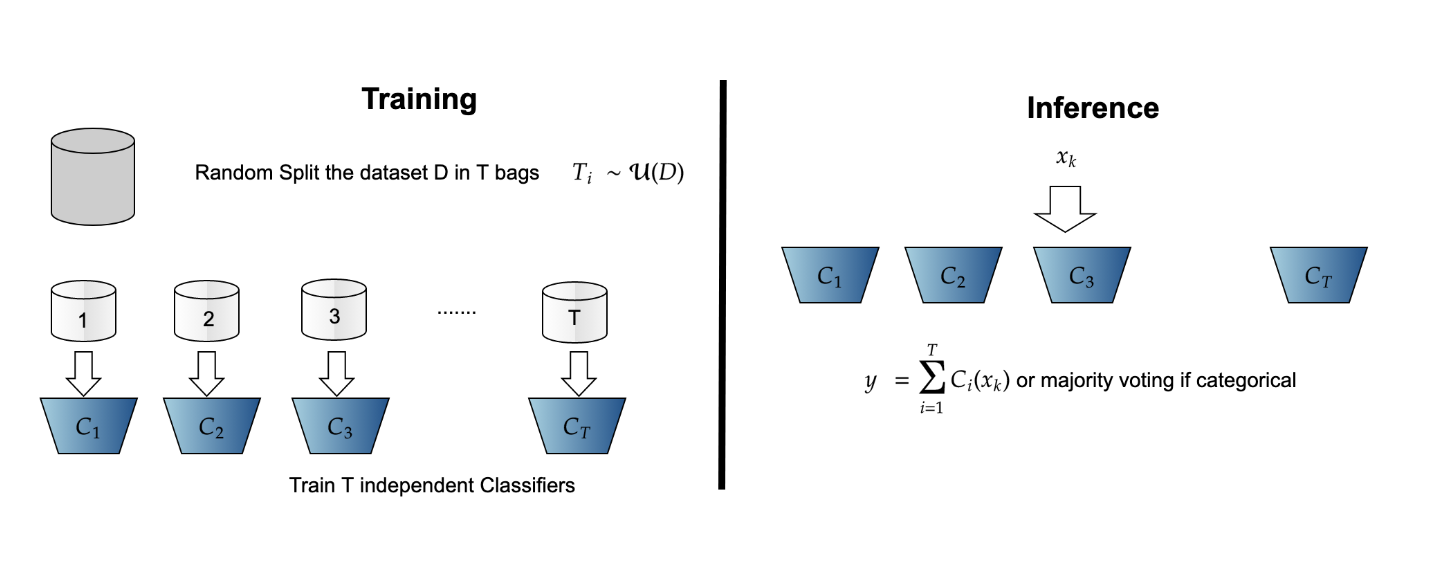
\includegraphics[width=0.8\linewidth]{Images/ensembles/Bagging.png}
    \caption{Approccio del Bagging}
\end{figure}

\begin{ex}[Dimostrazione]
  Supponiamo che ogni classificatore abbia come funzione $y = f_i(x) + e_i$ dove $e$ è l'errore.
  L'errore medio di $M$ classificatori sul dataset $D$ è:
  \[
    \mathcal{E}_{AV} = \frac{1}{M} \sum_{i=1}^{M} E_D[e_i]
  \]
  Invece, la predizione col bagging:
  \[
    y_{\text{bagged}} = \frac{1}{M} \sum_{i=1}^{M} f_i(x) + e_i(x)
  \]
  Quindi, l'errore medio del classificatore bagged è:
  \[
    \mathcal{E} = E_D\left[ \frac{1}{M} \sum_{i=1}^{M} e_i(x) \right]
  \]
\end{ex}

\section{Boosting}
Il boosting parte da un dataset $D$ e addestra sequenzialmente dei classificatori $f_i$, concentrandosi sugli errori commessi dai classificatori precedenti.
Addestrato per correggere con successo gli errori dei modelli precedenti.

\begin{ex}[Approccio]
  Assegna a ogni $x_k \in D$ peso uguale $w_k = \frac{1}{N}$, poi succesivamente iterare con $i$ da $1$ a $M$, quindi il numero di stage del boosting:
  \begin{enumerate}
    \item Genera un nuovo dataset $D_i$ da $D$ usando i pesi $\{w^i_k\}_{k=1}^N$ come probabilità di scelta per ogni record $x$.
    \item Allena l'i-esimo classificatore $f_i$ su $D_i$ e misura l'accuratezza $\alpha_i$.
    \item Se $x_k$ è stato classificato erroneamente, incrementane il peso per la fase successiva $(w_i+1)$ e normalizza nuovamente i pesi.
  \end{enumerate}
  La decisione finale equivale a:
  \[
    y(x_{\text{new}}) = sign\left( \sum_{i}^M \alpha_i f_i(x_{\text{new}}) \right)
  \]
\end{ex}
Ogni classificatore nella catena di boosting deve avere un'accuratezza superiore a $0.5$. \\
Agli elementi classificati erroneamente viene attribuito un peso maggiore e aumenta la probabilità che vengano campionati man mano che la catena si allunga.
Catene più lunghe tendono ad aumentare l'accuratezza, ma anche il rischio di overfitting.

\section{AdaBoost}
L'obiettivo è eliminare il campionamento dagli algoritmi di boosting convenzionali, sfruttando il peso del campione nella valutazione dell'errore della singola fase. \\
L'errore di un classificatore alla fase $k$ è: 
\[
  \epsilon_k = \sum_{i=1}^N w_k^i \nVDash (f_k(x^i) \neq y^i)
\]
Dopo ogni fase degli algoritmi di boosting, i pesi dei campioni vengono modificati, tramite la \textbf{trust} $\alpha_k = \log{\frac{1 -\epsilon_k}{\epsilon}}$:
\begin{itemize}
  \item Il peso degli elementi classificati erroneamente viene aumentato: $w_{k+1}^i = w_k^i \exp^{+\alpha_k}$.
  \item Il peso degli elementi classificati correttamente viene diminuito: $w_{k+1}^i = w_k^i \exp^{-\alpha_k}$
\end{itemize}
Ciò significa che, in ogni fase, gli elementi classificati in modo errato sono più importanti per il classificatore corrente e
ciascun classificatore, in ogni fase, deve comunque raggiungere un'accuratezza superiore a $0.5$, in termini di accuratezza pesata, altrimenti la catena si riavvia.

\begin{figure}[!htb]
    \centering
    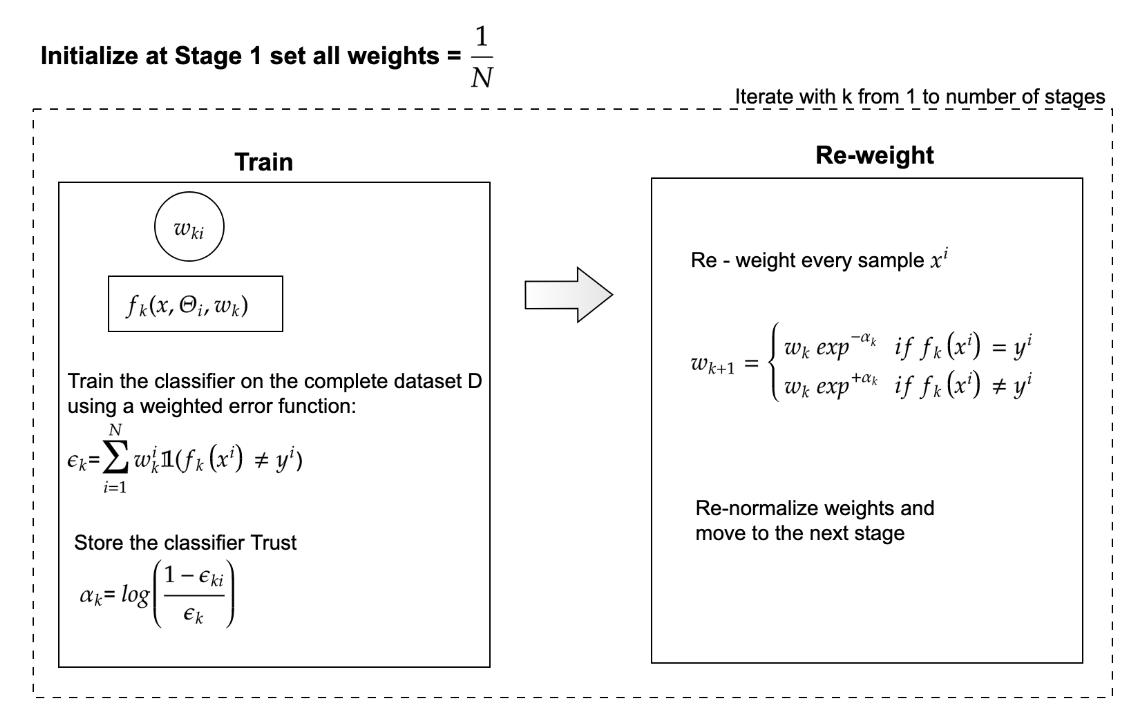
\includegraphics[width=0.6\linewidth]{Images/ensembles/AdaBoost.png}
    \caption{Approccio del Bagging}
\end{figure}

La regola decisionale finale è una somma ponderata delle risposte individuali:
\[
  y^i = sign\left( \sum_{k=1}^M \alpha_k f_k(x^i) \right)
\]
